\section{Checking the contribution of each component}
\label{sec:components}
The previous models form a sequence of choices, so a faster final calculation does not identify which choice supplies the saving. We compare ten methods on fourteen fresh batches from seven known graph structures and then disable individual learned decisions while keeping the other stages unchanged. Every method uses the same targets and prescribed basis. All 420 reductions in the first comparison and all 96 additional decision controls pass exact coefficient checks.

The native-choice total is 66.035 seconds, using sums of three-run batch medians. Table~\ref{tab:component-common} shows the complete strategies relative to that control. The result through worker selection takes 46.777 seconds, but this saving includes fixed seed settings as well as learned decisions. The equation, seed, and row filters increase time on this particular target pattern. Earlier savings on other targets remain separate results.

\begin{table}[!htbp]\centering\small
\caption{Component comparison on the same fourteen batches. Complete times include decisions, exact checks, and recovery. The first three rows retain preceding stages.}
\label{tab:component-common}
\begin{tabular}{@{}lrl@{}}\toprule
Method & Complete time (s) & Change from native\\\midrule
Graph-strategy model & 61.779 & 6.4\% less time\\
Through seed expansion & 49.309 & 25.3\% less time\\
Through worker selection & 46.777 & 29.2\% less time\\
Equation filter & 72.446 & 9.7\% more time\\
Seed filter & 70.241 & 6.4\% more time\\
Row model & 105.500 & 59.8\% more time\\
\bottomrule\end{tabular}\end{table}

\begin{table}[!htbp]\centering\small
\caption{The added learned decision, with other stages held fixed. Each row uses the subset on which that decision is enabled. Fixed settings were selected before this test.}
\label{tab:isolated-choices}
\begin{tabular}{@{}lrrrl@{}}\toprule
Decision & Batches & Fixed (s) & Learned (s) & Change\\\midrule
Graph choice & 6 & 51.448 & 50.188 & 2.4\% less time\\
Seed expansion & 6 & 41.030 & 41.093 & 0.2\% more time\\
Worker count & 4 & 24.232 & 25.555 & 5.5\% more time\\
\bottomrule\end{tabular}\end{table}

The isolated controls in Table~\ref{tab:isolated-choices} show why complete-time gains need a fixed comparison. On these batches, graph choice saves a small amount, while the added seed and worker choices increase time. Figure~\ref{fig:component-controls} presents both comparisons. These results motivate replacing the sequence of selectors with the single cost policy in the next section.

\begin{figure}[tbp]\centering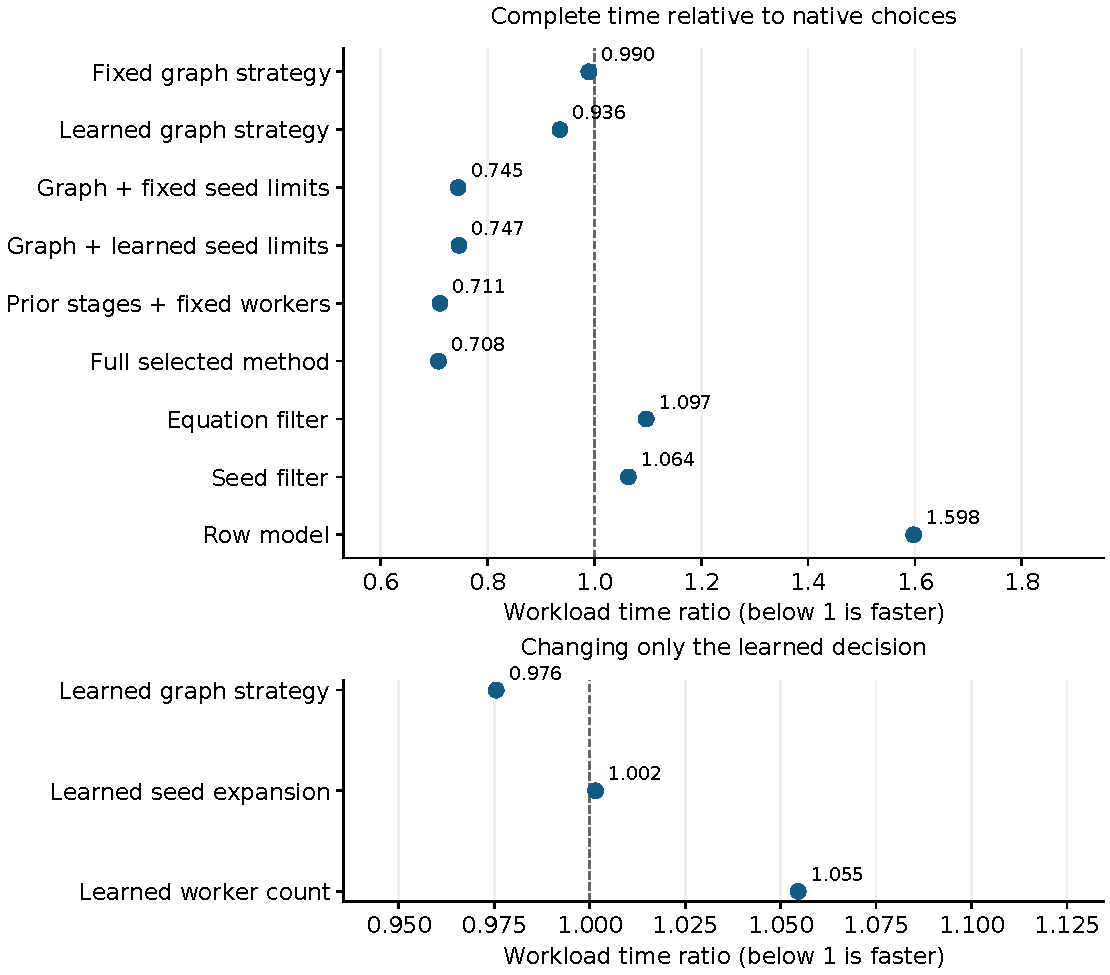
\includegraphics[width=\linewidth]{paper_figures/component_ablation.pdf}
\caption{Complete strategies and their added learned decisions. The upper panel uses all fourteen batches. The lower panel changes one learned decision on its enabled subset. Both show ratios of summed batch medians and retain the equal-time reference.}
\label{fig:component-controls}\end{figure}

\subsection{Connected scattering and bounded higher-loop tests}
We also construct connected four-point ladders and boxes with bubble subgraphs, defined in Appendix~\ref{app:higher-scattering}. The two completed three-loop bubble-box profiles take 10.538 seconds with restricted initialization and native equation choices, compared with 7.468 seconds with the frozen equation filter. This is 29.1\% less time under the same initialization. The complete strategy selectors otherwise retain native choices on these previously unsupported graph structures.

The bounded four- through six-loop probes identify separate costs and limits. Four-loop initialization exceeds the initial short time allowance. Five-loop attempts exceed the memory allowance, and the six-loop four-point representation requires 39 inverse propagators, above the tested executable's 31-entry limit. Later runs produce a four-loop bubble-box reference and reproduce its coefficients with enlarged seeds. Three native repetitions have median time 465.329 seconds. Two completed filtered repetitions take 520.336 and 551.161 seconds, each requiring native recovery after an insufficient equation set. Only these two filtered repetitions complete, so this diagnostic supplies no matched three-run speedup estimate. The incomplete attempt is excluded from timing results.

The new work therefore addresses both preparation and the learned choice. A complete four-loop reduction is established for the stated bubble-box family, while the failed larger-family probes supply no speedup claim. The vacuum recurrence used elsewhere in this paper does not determine the scattering coefficients, as explained in Appendix~\ref{app:higher-scattering}.
